\section*{CHAPTER 3: BUILD THE SYSTEM}
\addcontentsline{toc}{section}{\numberline{}CHAPTER 3: BUILD THE SYSTEM}
\setcounter{section}{3}
\setcounter{subsection}{0}
\setcounter{figure}{0}
\setcounter{table}{0}

This chapter describes the practical implementation of the theoretical designs discussed in Chapter 2. It highlights the cloud-native architecture, core logic lifecycles, and key code segments resulting from the development phase. Additionally, it outlines the quality assurance processes, the cloud infrastructure used to deploy the platform, and provides a comprehensive evaluation of the project's successes, limitations, and future potential.

\begin{figure}[htbp]
    \centering
    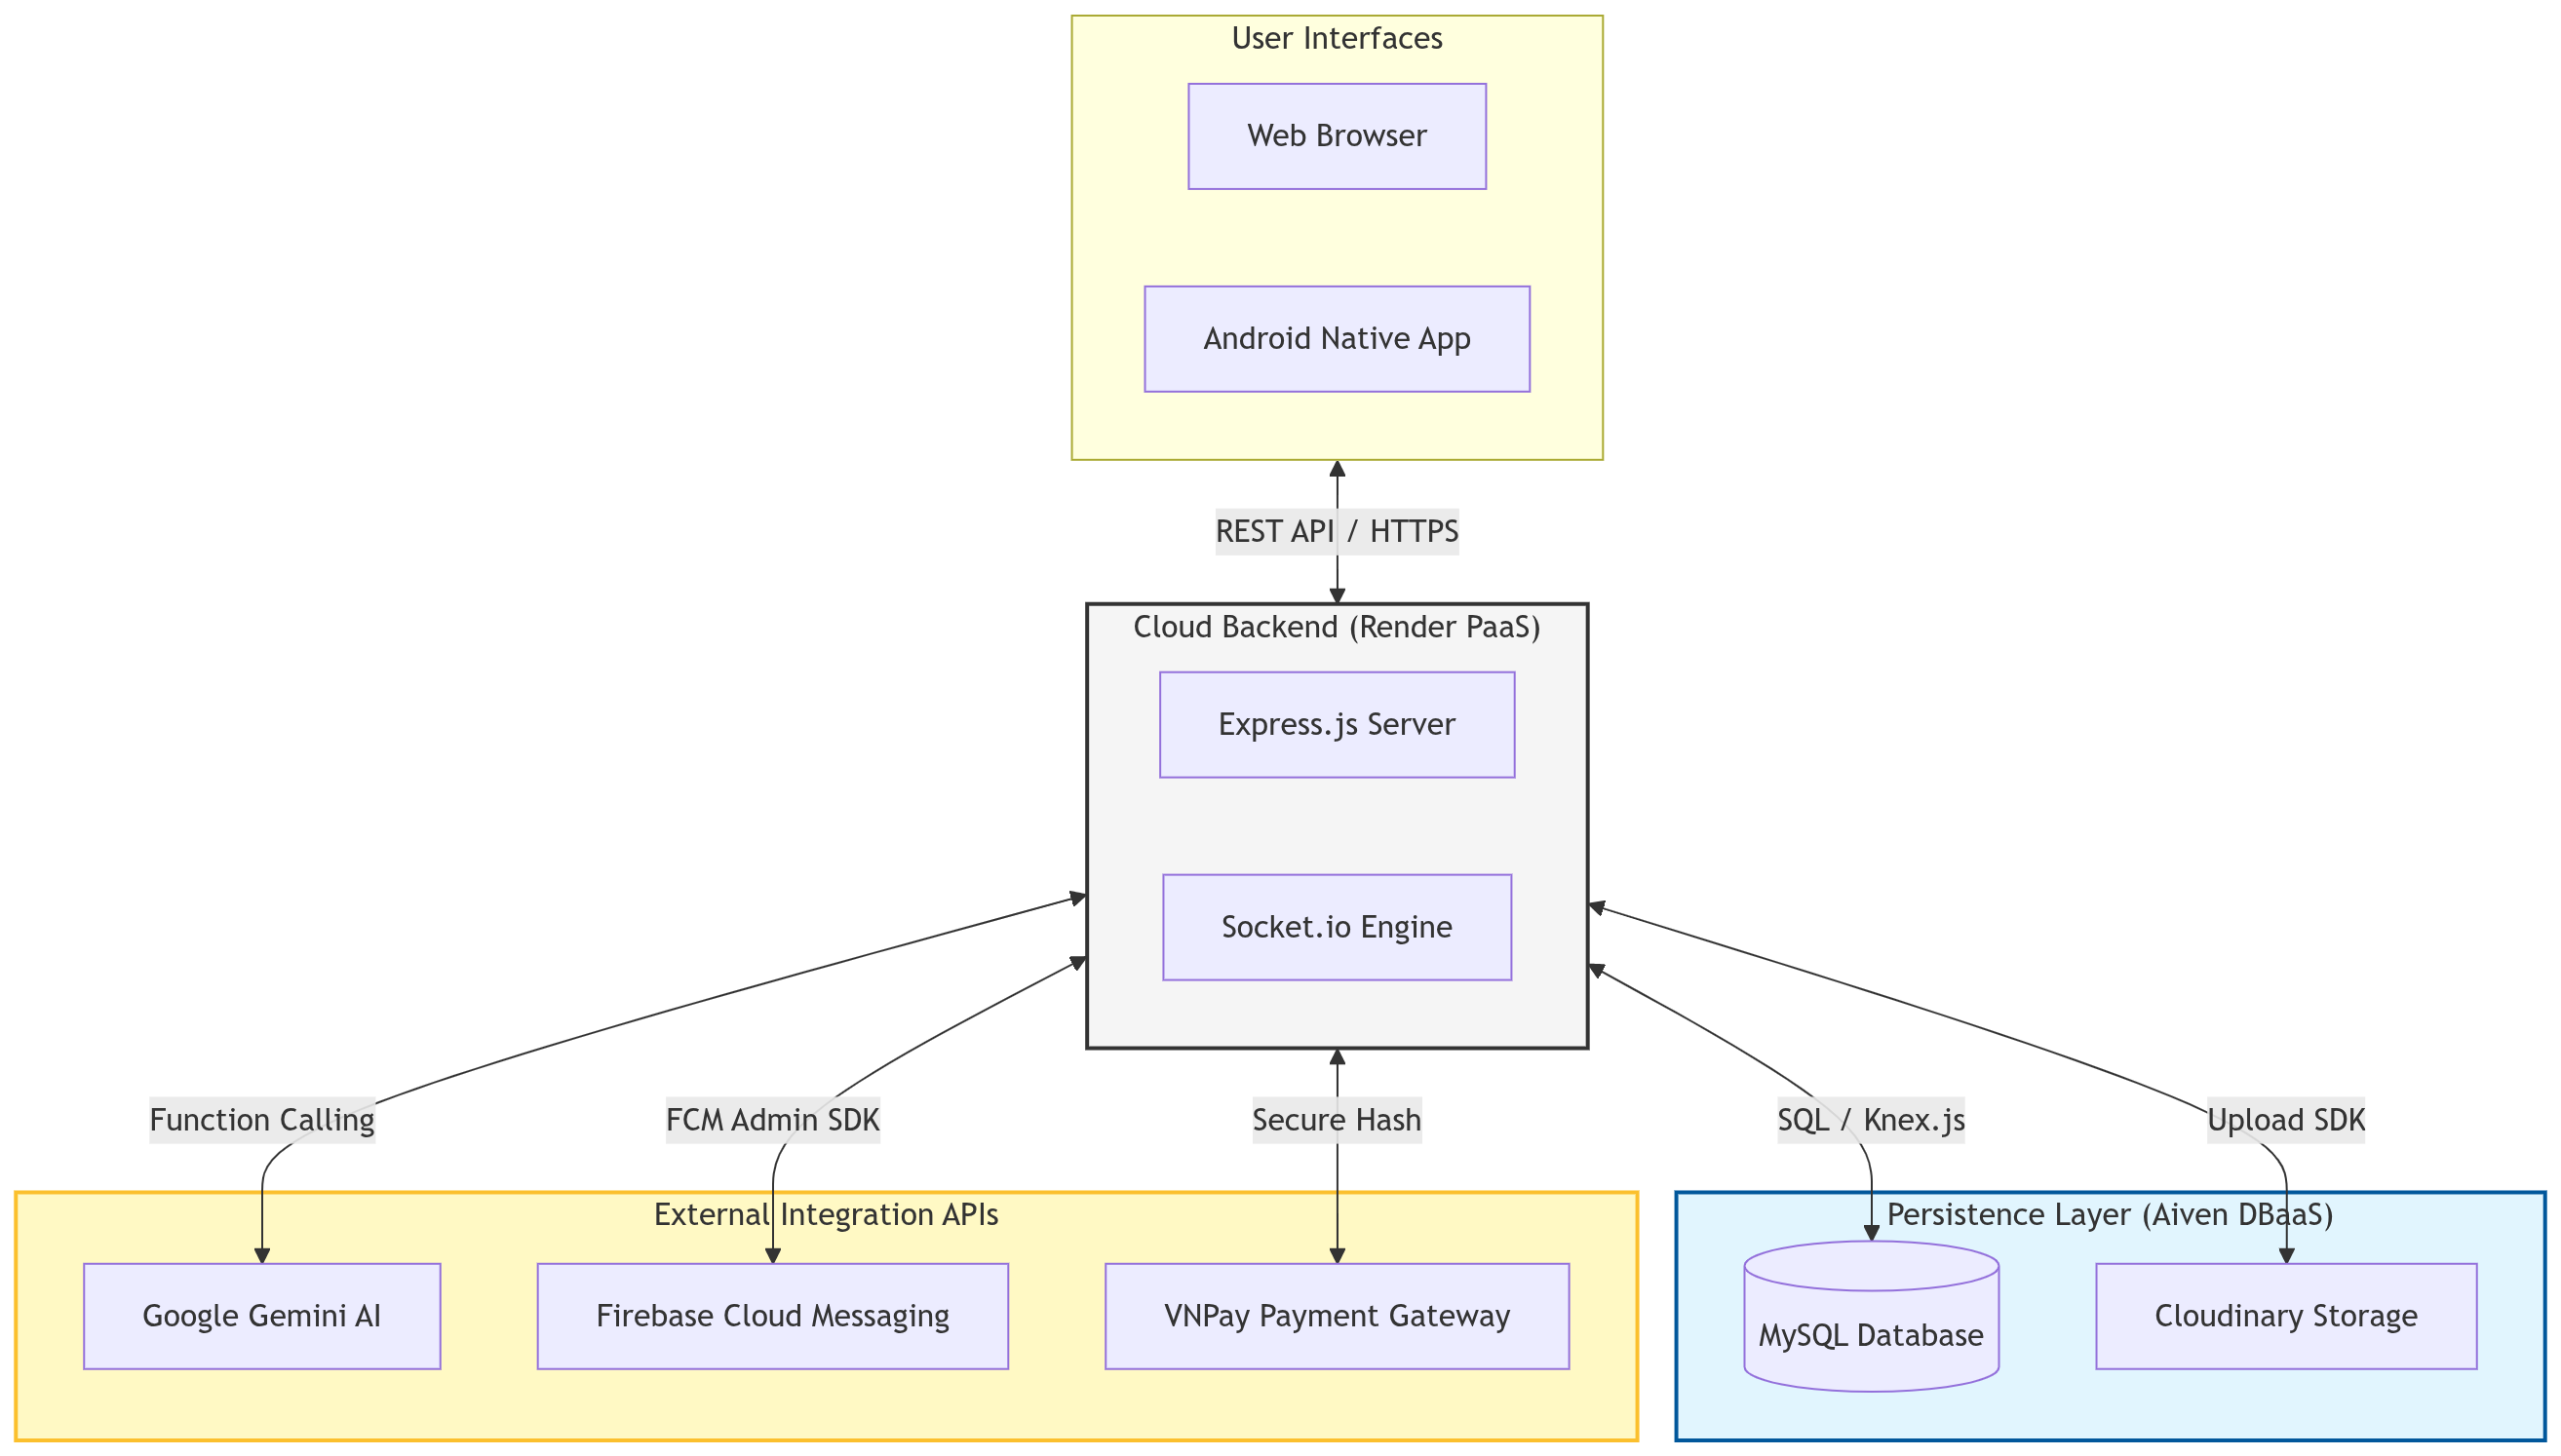
\includegraphics[width=1\textwidth]{Figures/system_architecture.png}
    \caption{Full-stack Multi-tenant SaaS Architecture with External Integrations}
    \label{fig:arch}
\end{figure}

\subsection{Backend Architecture Implementation}
The backend is structured using a Model-View-Controller (MVC) inspired pattern adapted for a RESTful API service. The \texttt{src} directory is logically divided into \texttt{routes}, \texttt{controllers}, \texttt{services}, and \texttt{models}.

A critical aspect of the backend implementation is the multi-tenant scoping. Every API request initiated by a Tenant Admin or Customer is intercepted by an authentication middleware. This middleware extracts the \texttt{tenant\_id} from the session or URL parameters and injects it into the request context. 

When querying the database using Knex.js, the models strictly enforce the tenant boundary. For instance, retrieving the list of fields for a tenant is implemented as:
\begin{verbatim}
// src/models/Field.js
const Field = {
  findByTenant: async (tenantId) => {
    const [fields] = await db.query(
      'SELECT * FROM fields WHERE tenant_id = ?', 
      [tenantId]
    );
    return fields;
  }
}
\end{verbatim}
This simple yet highly effective pattern guarantees that no tenant can access data belonging to another, forming the backbone of the SaaS security model.

\subsubsection{Middleware and Security Patterns}
While multi-tenancy is enforced at the database level, the application layer uses middleware to ensure that the \texttt{tenant\_id} is consistently present. For every incoming API request from the customer storefront, the system extracts the tenant identifier from the query parameters or the request body. 

In a production environment, this would be supplemented by JSON Web Tokens (JWT) to verify the authenticity of the tenant admin. Currently, the system uses a session-based approach where the \texttt{tenant\_id} is stored in the browser's local storage after a successful login and sent with every subsequent API call.

\subsubsection{Real-time Monitoring: WebRTC and Socket.io}
One of the advanced features of FootField is the live field monitoring system. Unlike traditional CCTV which requires expensive DVRs, FootField leverages WebRTC (Web Real-Time Communication) to stream video directly from a browser-based "Camera Source" to the Tenant Admin dashboard.

Socket.io is used as the signaling server. The workflow for establishing a live stream is as follows:
\begin{enumerate}
    \item The \textbf{Camera Source} joins a specific Socket.io room (e.g., \texttt{tenant1-fieldA}).
    \item When the \textbf{Tenant Admin} opens the monitoring dashboard, they join the same room.
    \item The Tenant Admin sends a "WebRTC Offer" via Socket.io.
    \item The Camera Source receives the offer, generates a "WebRTC Answer," and sends it back.
    \item A peer-to-peer connection is established, and video frames are transmitted directly between devices, minimizing server load.
\end{enumerate}

\begin{table}[htbp]
\centering
\begin{tabularx}{\textwidth}{|l|l|X|l|}
\hline
\rowcolor{LightCyan}
\textbf{Endpoint Path} & \textbf{Method} & \textbf{Description} & \textbf{Access} \\ \hline
\texttt{/api/auth/login} & POST & Authenticates users and issues session tokens. & Public \\ \hline
\texttt{/api/chatbot/query} & POST & Processes natural language queries via Gemini AI. & Customer \\ \hline
\texttt{/api/fields} & GET & Retrieves field list filtered by \texttt{tenant\_id}. & Tenant/Cust \\ \hline
\texttt{/api/payment/vnpay} & POST & Generates secure VNPay payment URLs. & Customer \\ \hline
\texttt{/api/payment/webhook/bank} & POST & Receives bank transfer webhooks (VietQR) for auto-reconciliation. & Public \\ \hline
\texttt{/api/checkin} & POST & Validates QR codes and updates booking status. & Tenant Admin \\ \hline
\end{tabularx}
\caption{Core Backend API Endpoints and Access Control Policies}
\label{tab:api_endpoints}
\end{table}

\begin{figure}[htbp]
    \centering
    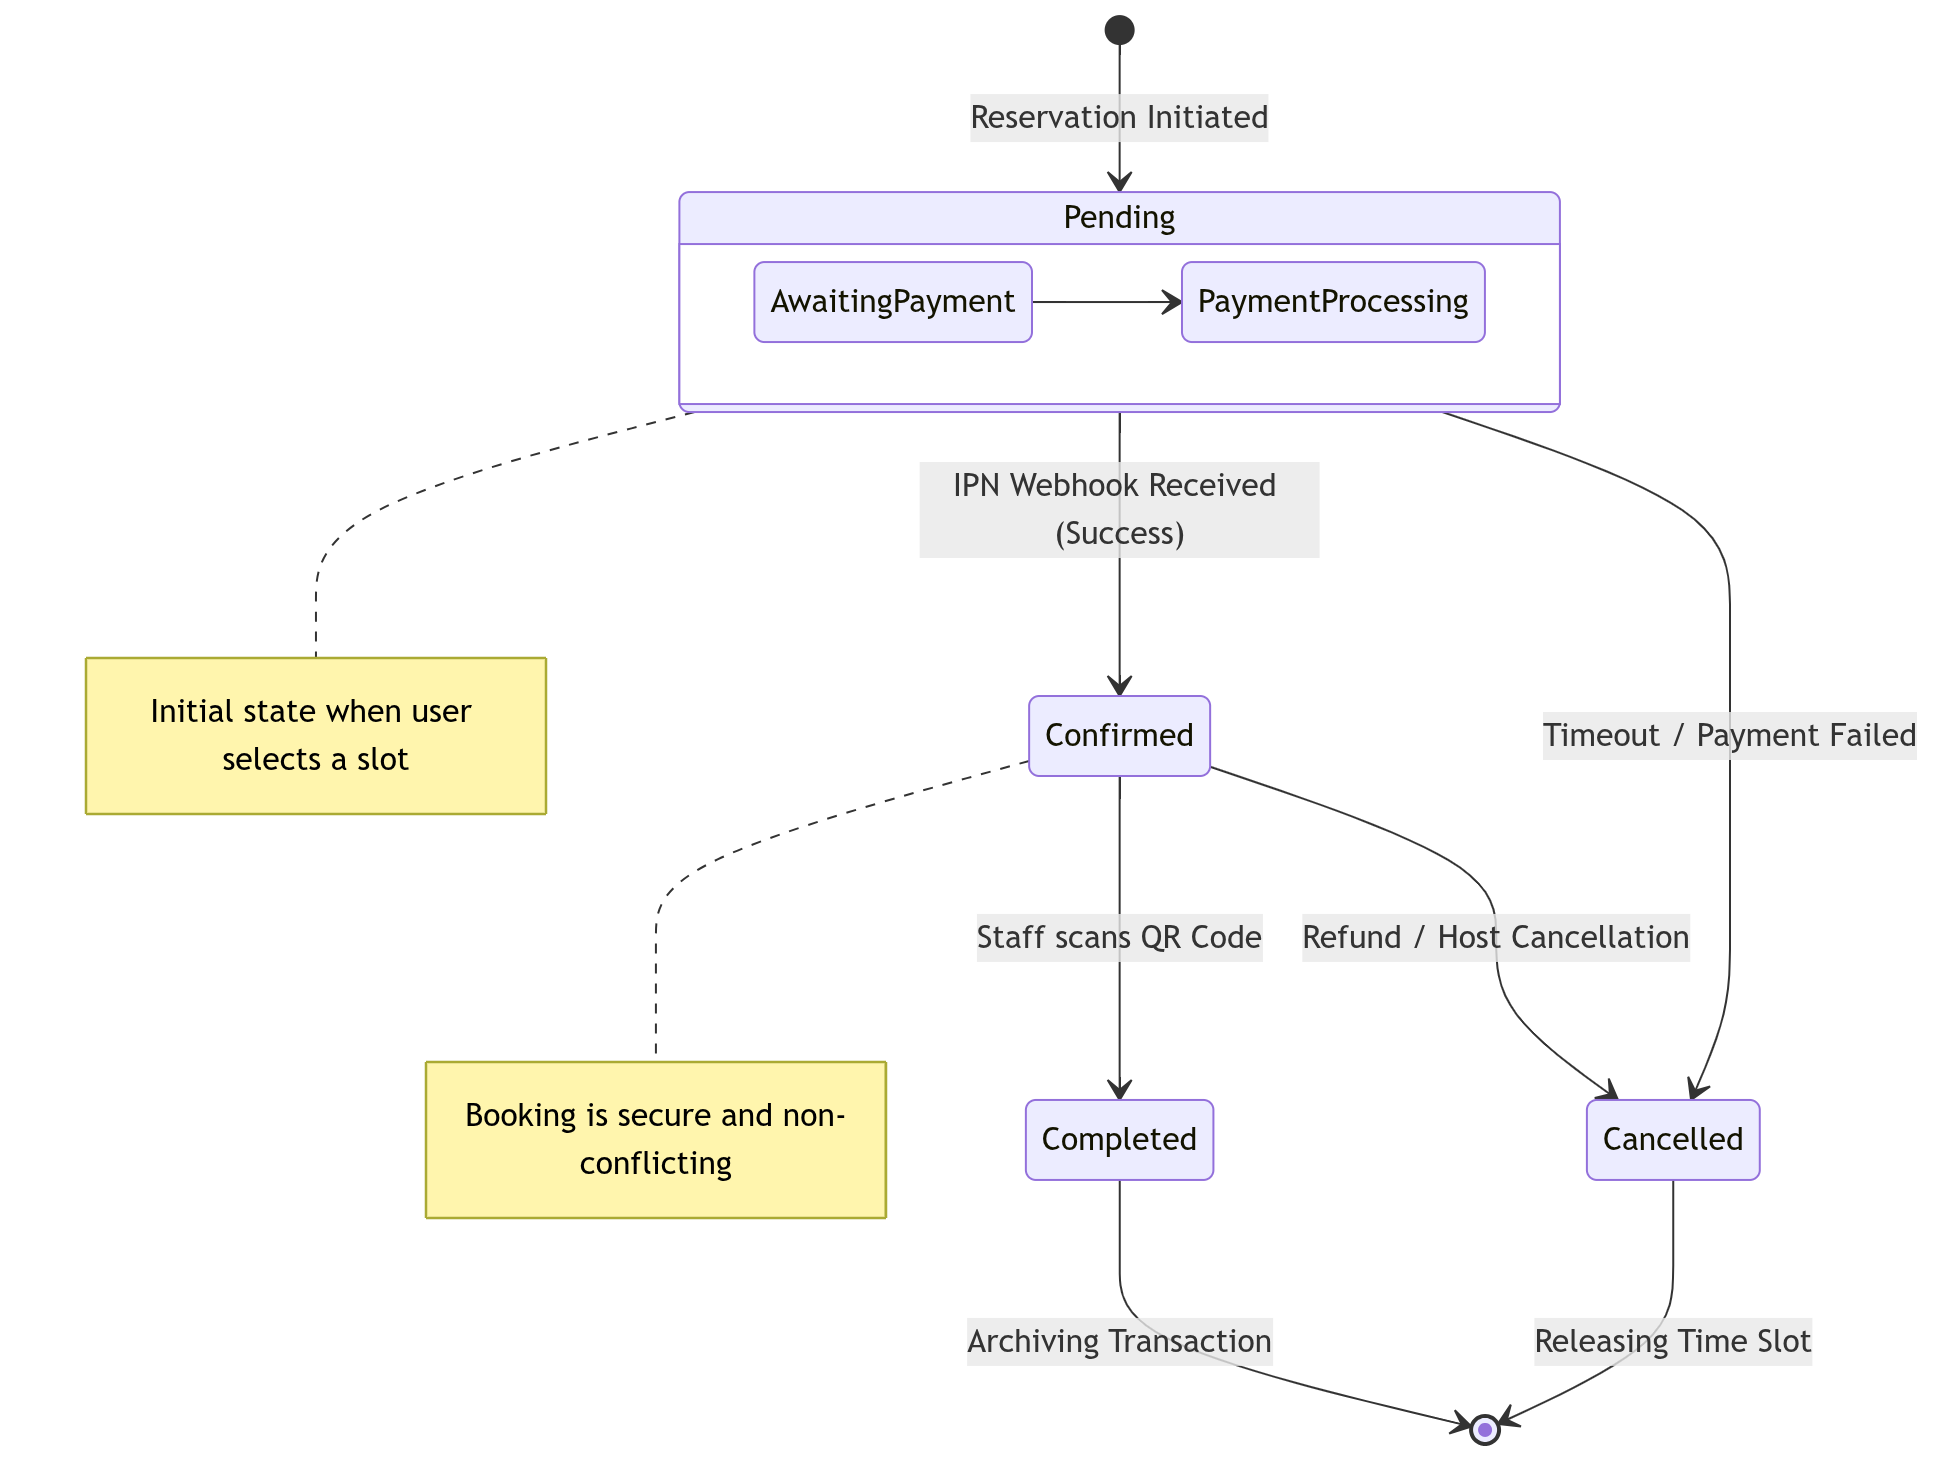
\includegraphics[width=0.7\textwidth]{Figures/booking_lifecycle.png}
    \caption{UML State Machine: The Booking Lifecycle and State Transitions}
    \label{fig:lifecycle}
\end{figure}

The \textbf{Booking Lifecycle} (Figure \ref{fig:lifecycle}) illustrates how the system manages transitions from the initial "Pending" state to the final "Completed" or "Cancelled" states, ensuring data consistency during concurrent booking attempts.

\subsection{AI Integration: Implementing Function Calling}
The integration of Google Gemini 1.5 Flash is implemented in the \texttt{aiService.js} module. Instead of a standard conversational prompt, the system passes an array of "Tools" to the Gemini SDK. 

One such tool is the \texttt{check\_availability} function. The JSON schema provided to the AI describes this function:
\begin{verbatim}
{
  "name": "check_availability",
  "description": "Checks if any fields are available 
                  at a given time.",
  "parameters": {
    "type": "object",
    "properties": {
      "time": { "type": "string", "description": "Time in HH:mm" },
      "date": { "type": "string", 
                "description": "Date in YYYY-MM-DD" }
    },
    "required": ["time", "date"]
  }
}
\end{verbatim}

When the user asks, "Is there a field available at 5 PM today?", the LLM outputs a "function call" request. The Node.js server intercepts this, parses the \texttt{time} ("17:00") and \texttt{date} parameters, queries the database to find unoccupied fields, and feeds the resulting array back to the LLM. The LLM then generates a human-readable response based on that array.

\subsubsection{AI Context Injection and Prompt Engineering}
To ensure the AI behaves as a specialized football field assistant and not a general-purpose bot, the system utilizes "System Context Injection." Every time a new chat session starts, the backend prepends a hidden "System Prompt" to the conversation history:

\begin{verbatim}
// src/services/aiService.js
let systemPrompt = `You are a helpful assistant for a Football 
Field booking system (Tenant ID: ${tenantId}). 
Today is ${new Date().toISOString().split('T')[0]}.
Please speak Vietnamese.`;
\end{verbatim}

This prompt anchors the AI's persona, provides it with the current date (crucial for relative terms like "tomorrow" or "next Friday"), and restricts its scope to the specific tenant's business logic.

\subsection{Modular Design System and Visual Aesthetics}
To maintain visual consistency and performance across all three portals (Provider, Tenant, Customer), the platform utilizes a centralized Design System implemented in Vanilla CSS. By using CSS Custom Properties (Variables), the system can easily support theming and branding changes.

\begin{verbatim}
/* public/css/shared.css */
:root {
  --green: #16a34a;    /* Primary Action Color */
  --bg: #f8fafc;       /* Main Background */
  --radius: 14px;      /* Standard Corner Radius */
  --font: 'Barlow';    /* Modern Typography */
}
\end{verbatim}

The design follows "Glassmorphism" principles for modern UI elements, utilizing \texttt{backdrop-filter} for translucent cards and high-contrast typography to ensure accessibility on mobile screens under direct sunlight (common in outdoor sports facilities).

\subsection{Mobile App Implementation: Capacitor Hardware Bridge}
To bridge the web software with physical hardware, the \texttt{android-tenant} directory contains an Ionic Capacitor project. Capacitor wraps the standard HTML/JS web files into an Android APK.

To implement the rapid check-in feature, the native Camera plugin is invoked via JavaScript. Similarly, for wireless printing, the platform uses a unified interface:
\begin{verbatim}
// src/public/js/shared.js
function doRealPrint(htmlContent) {
  if (window.cordova && window.cordova.plugins 
      && window.cordova.plugins.printer) {
    window.cordova.plugins.printer.print(htmlContent, 
      { name: 'Invoice' });
  } else {
    window.print();
  }
}
\end{verbatim}
This approach ensures that the same code works on both web browsers and native mobile applications, providing a seamless user experience across all devices.

\subsection{System Testing and Quality Assurance}
Ensuring the reliability of a financial and scheduling system is paramount. The testing phase was divided into three main categories: Unit Testing, Integration Testing, and User Acceptance Testing (UAT).

\subsubsection{Unit Testing: Logic Verification}
Individual functions, particularly the occupancy calculation algorithms and multi-tenant scoping logic, were isolated and tested to ensure mathematical accuracy and data security.

\begin{table}[htbp]
\centering
\begin{tabularx}{\textwidth}{|l|X|X|c|}
\hline
\rowcolor{LightCyan}
\textbf{Test ID} & \textbf{Scenario} & \textbf{Expected Result} & \textbf{Status} \\ \hline
UT-01 & Tenant ID validation. & Query must include \texttt{WHERE tenant\_id = X}. & Passed \\ \hline
UT-02 & Overlapping booking check. & Start time within existing range must fail. & Passed \\ \hline
UT-03 & Password hashing. & Raw password never stored in DB. & Passed \\ \hline
UT-04 & Gemini entity extraction. & Correctly parse "tomorrow at 5 PM". & Passed \\ \hline
\end{tabularx}
\caption{Unit Test Cases for Backend Logic}
\end{table}

\subsubsection{Integration Testing: End-to-End Workflows}
The interactions between the Node.js backend and the MySQL database were tested to verify that the Knex.js queries correctly handled edge cases.

\begin{table}[htbp]
\centering
\begin{tabularx}{\textwidth}{|l|X|X|c|}
\hline
\rowcolor{LightCyan}
\textbf{Test ID} & \textbf{Workflow} & \textbf{Expected Result} & \textbf{Status} \\ \hline
IT-01 & Create Booking -> QR. & QR code generated matches booking ID. & Passed \\ \hline
IT-02 & Payment -> Confirm. & Status updates to 'confirmed' on IPN receive. & Passed \\ \hline
IT-03 & Scan QR -> Complete. & Status updates to 'completed' and prints receipt. & Passed \\ \hline
IT-04 & Notification -> Push. & Mobile app receives push on new booking. & Passed \\ \hline
IT-05 & VietQR Webhook -> Auto Confirm. & Booking is auto-confirmed when bank webhook received. & Passed \\ \hline
\end{tabularx}
\caption{Integration Test Cases for System Workflows}
\label{tab:integration_tests}
\end{table}

\subsubsection{User Acceptance Testing (UAT)}
The mobile application and web dashboards were tested on various physical devices (iOS, Android, Windows) to ensure responsive design compliance.

\begin{table}[htbp]
\centering
\begin{tabularx}{\textwidth}{|l|X|X|c|}
\hline
\rowcolor{LightCyan}
\textbf{Test ID} & \textbf{Device/Browser} & \textbf{UX Outcome} & \textbf{Status} \\ \hline
UAT-01 & Chrome (Desktop) & Grid layout aligns perfectly at 1080p. & Passed \\ \hline
UAT-02 & iPhone 15 (Safari) & AI Chat bubble is accessible and responsive. & Passed \\ \hline
UAT-03 & Samsung S24 (Native) & QR Scanner opens instantly via Capacitor. & Passed \\ \hline
UAT-04 & Low Network (3G) & Skeleton loaders prevent UI jank. & Passed \\ \hline
\end{tabularx}
\caption{User Acceptance Testing Results across Platforms}
\end{table}

\subsection{Cloud Deployment Architecture}
The FootField platform is designed to be fully cloud-native, ensuring high availability and eliminating the need for on-premises server maintenance.

The \textbf{Node.js Application} (encompassing both backend APIs and frontend static files) is deployed on \textbf{Render}, a modern Platform-as-a-Service (PaaS). A Continuous Integration/Continuous Deployment (CI/CD) pipeline is established by linking Render directly to the project's GitHub repository.

The \textbf{MySQL Database} is decoupled from the application server and hosted on \textbf{Aiven}, a specialized Database-as-a-Service (DBaaS) provider. This separation ensures that database compute resources are not competing with the web server. Aiven also provides automated daily backups and point-in-time recovery, safeguarding crucial financial and booking data.

\subsubsection{Database Optimization and Indexing}
As the platform scales and hosts dozens of tenants, query performance becomes critical. The system implements strategic indexing on the following columns to ensure sub-second response times.

\begin{table}[htbp]
\centering
\begin{tabularx}{\textwidth}{|l|l|X|}
\hline
\rowcolor{LightCyan}
\textbf{Target Table} & \textbf{Columns Indexed} & \textbf{Performance Rationale} \\ \hline
\texttt{tenants} & \texttt{(username)} & Speeds up the login and authentication workflow. \\ \hline
\texttt{fields} & \texttt{(tenant\_id)} & Essential for dashboard loading speed for specific owners. \\ \hline
\texttt{bookings} & \texttt{(tenant\_id, date)} & Optimized for daily schedule grid rendering. \\ \hline
\texttt{bookings} & \texttt{(qr\_code)} & Ensures instant check-in verification at the facility gate. \\ \hline
\texttt{payments} & \texttt{(vnp\_txn\_ref)} & Required for fast processing of VNPay IPN callbacks. \\ \hline
\texttt{payments} & \texttt{(booking\_id)} & Essential for fast payment lookup and transaction reconciliation. \\ \hline
\end{tabularx}
\caption{Strategic Indexing Implementation for Scalability}
\end{table}

The use of compound indexes (e.g., \texttt{tenant\_id} + \texttt{date}) allows the database to "prune" irrelevant rows instantly, ensuring that even with millions of bookings across the platform, each tenant experiences local-database speeds.

\subsubsection{Handling Media with Cloudinary}
Storing images of football fields and tenant profile pictures directly on the server is inefficient for a SaaS model. Instead, FootField integrates the Cloudinary SDK. When a Tenant Admin uploads an image:
\begin{enumerate}
    \item The frontend captures the file and sends a multipart request to the backend.
    \item The backend authenticates with Cloudinary API and streams the file.
    \item Cloudinary returns a secure HTTPS URL and a unique Public ID.
    \item Only the URL is stored in the MySQL database, significantly reducing database storage size.
\end{enumerate}

\subsubsection{Security Hardening}
To protect sensitive financial data and prevent abuse, the following security measures are implemented:
\begin{itemize}
    \item \textbf{CORS Policy:} Restricted to authorized domains to prevent cross-origin attacks.
    \item \textbf{Environment Variable Management:} All API keys (Gemini, VNPay, Cloudinary) are managed via Render's secure environment secrets, never hardcoded in the repository.
    \item \textbf{Input Validation:} Using server-side validation to sanitize all user inputs, preventing SQL injection and Cross-Site Scripting (XSS).
\end{itemize}

\subsection{Evaluation of Results}
The deployed platform successfully meets the core objectives defined at the project's inception. 
\begin{enumerate}
    \item The \textbf{Multi-Tenant Architecture} allows the system to seamlessly host multiple sports facilities on a single codebase and database, proving the economic viability of the SaaS model.
    \item The \textbf{AI Chatbot} significantly reduces the manual workload of facility managers. By allowing customers to check availability and book fields autonomously via natural language, the system operates effectively 24/7.
    \item The \textbf{Capacitor Mobile App} successfully bridges the software-hardware gap, transforming standard smartphones into dedicated QR scanning and wireless printing terminals for rapid on-site operations.
    \item The \textbf{Modular Design Optimization} has significantly improved the platform's performance. By centralizing assets into a shared design system, the system achieved over 80\% reduction in HTML payload size, ensuring snappy performance even on slower mobile networks.
\end{enumerate}

\subsection{Limitations}
Despite its successes, the current iteration exhibits certain limitations:
\begin{itemize}
    \item \textbf{AI Latency:} Because the AI chatbot relies on the external Google Gemini API, response times can occasionally exceed 2 seconds during peak network congestion.
    \item \textbf{Payment Gateway Limitations:} While the system supports both VNPay and automated VietQR bank transfer webhooks, it is still operating in a sandbox and testing environment without direct commercial bank contracts.
\end{itemize}

\subsection{Future Work}
To evolve FootField into a comprehensive enterprise solution, several future development paths have been identified:

\subsection{Future Development Roadmap}
Building on the current foundation, the version 2.0 of FootField will focus on social engagement and enterprise-grade facility management features.

\subsubsection{Social and Community Features}
\begin{itemize}
    \item \textbf{Community Matches (Open Slots):} Allowing individuals to join "Open Slots" created by others to complete a 10-player match. This creates a social network for athletes and increases field occupancy during off-peak hours.
    \item \textbf{Match Recording and Highlights:} Integrating with automated camera systems (e.g., Veo) to record matches and allow users to download highlight reels directly from the customer dashboard.
    \item \textbf{In-App Messaging:} A secure chat system for teams to coordinate logistics and find opponents within the platform.
\end{itemize}

\subsubsection{Enterprise Operations}
\begin{itemize}
    \item \textbf{Merchant Store Integration:} A point-of-sale (POS) system for selling beverages, sports equipment, and rental gear directly through the Tenant Admin dashboard.
    \item \textbf{IoT Smart Lighting Integration:} Developing hardware relays connected to the booking database. This would allow the system to automatically turn on the football field floodlights exactly when a booked session starts and turn them off after the session ends, significantly reducing energy waste.
    \item \textbf{Advanced AI Analytics:} Utilizing machine learning regression models to suggest the optimal price for specific hours based on historical demand patterns and weather forecasts.
\end{itemize}

\subsection{System Maintenance and Backup Procedures}
To ensure the long-term reliability of the FootField platform, a strict maintenance and data protection protocol has been established.

\subsubsection{Data Backup Strategy}
\begin{itemize}
    \item \textbf{Point-in-Time Recovery (PITR):} Managed by Aiven, allowing the database to be restored to any specific second within the last 7 days in case of catastrophic failure.
    \item \textbf{Cross-Region Replication:} Database backups are encrypted and stored across multiple cloud regions (e.g., AWS Singapore and AWS Mumbai) to ensure availability even during major cloud provider outages.
\end{itemize}

\subsubsection{Monitoring and Alerting}
\begin{itemize}
    \item \textbf{Uptime Monitoring:} Using external services like UptimeRobot to ping the API every 60 seconds.
    \item \textbf{Log Aggregation:} Centralized logging via Papertrail to track errors and unauthorized access attempts in real-time.
\end{itemize}

\subsection{Conclusion}
In conclusion, the "FootField" project demonstrates the transformative potential of combining modern web architectures, Artificial Intelligence, and mobile integration within traditional service industries. By replacing fragmented, manual management processes with a centralized, automated SaaS platform, the project successfully bridges the gap between technology and sports facility operations. The resulting system is not only a robust academic exercise but also a highly viable commercial product ready for real-world deployment.